\chapter{Métodos numéricos}
A partir de las ecuaciones (\ref{eqn:helmholz}) y (\ref{eqn:helmholzH}), se puede aplicar la aproximación de guiaje débil para despreciar el lado derecho de ambas ecuaciones a fin de ignorar el efecto cruzado entre componentes de los campos. Las ecuaciones resultantes son del tipo Helmholtz:
\begin{equation}
	\left[\nabla^2 + k_0^2 n^2(\textbf{r})\right]\Psi(\textbf{r}) = 0. \label{eqn:helmholtznum}
\end{equation}
La ecuación (\ref{eqn:helmholtznum}) es la base de todos los métodos numéricos utilizados en esta tesis.
\section{Expansión en modos normales \label{cap:eme}}
Este método numérico es útil cuando los sistemas fotónicos en estudio son invariantes en la dirección de propagación $z$. Esto es, $n(\textbf{r})\equiv n(x,y)$. La soluciones de la ecuación (\ref{eqn:helmholtznum}) se pueden expandir en ondas planas con perfiles transversales: $\Psi(\textbf{r}) = \Psi(x,y) \exp({i\beta z})$. Con ésto, cada modo transversal $\nu$ debe cumplir la siguiente ecuación a resolver numéricamente:
\begin{equation}
	\left[\nabla_\perp^2 + k_0^2 n^2(x,y)\right]\Psi_\nu(x,y) = \beta_\nu^2\Psi_\nu(x,y) \ , \quad\text{ con } \nabla_\perp^2 \equiv \frac{\partial^2}{\partial x^2} + \frac{\partial^2}{\partial y^2} \ .
	\label{eqn:eme}
\end{equation}
Y el campo total propagado es una combinación lineal de los modos $\Psi_\nu$: 
\begin{equation}
	\Psi(\textbf{r}) = \sum_\nu a_\nu \Psi_\nu(x,y) e^{i\beta_\nu z}, \quad\text{ con } a_\nu \propto \Psi_\nu(x,y) \cdot \Psi(x, y, z=0).
\end{equation}
En vez de integrar directamente la ecuación de valores propios (\ref{eqn:eme}), la estrategia será discretizar el espacio y aproximar al operador Laplaciano transversal $\nabla_\perp^2$ como una matriz, pues $$\frac{\partial^2 \Psi(x,y)}{\partial x^2} \sim \frac{\Psi[i+1,j]-2\Psi[i,j]+\Psi[i-1,j]}{\Delta x ^2}  \ .
$$
$\nabla^2_\perp \sim \hat{D}_{xx} \otimes I_y + I_x \otimes \hat{D}_{yy}$
La matriz es nula (\textit{sparse-like}) en las posiciones no diagonales más allá de un espacio, por lo que es posible optimizar el proceso de cómputo al utilizar la librería de Python \href{https://docs.scipy.org/doc/scipy/reference/sparse.linalg.html}{\color{magenta}\texttt{scipy.sparse.linalg}}, especialmente diseñada para el álgebra lineal de matrices de escasos elementos. El anexo \ref{sec:codigohelmholtz} contiene una implementación de este algoritmo en Python bajo \href{https://www.gnu.org/licenses/gpl-3.0.html}{\color{magenta}licencia GNU GPL v3}.

En la Figura \ref{fig:emenumerror} se valida el método numérico mediante comparación con las soluciones analíticas obtenidas en la subsección \ref{cap:solslabTETM}. La complejidad del problema es del orden $O(N^2)$ debido a la construcción de las matrices de $N\times N$, lo que se refleja en la dependencia del tiempo de ejecución en función del paso $\Delta x \equiv \frac{L}{N-1}$.


\begin{figure}[H]
	\centering
	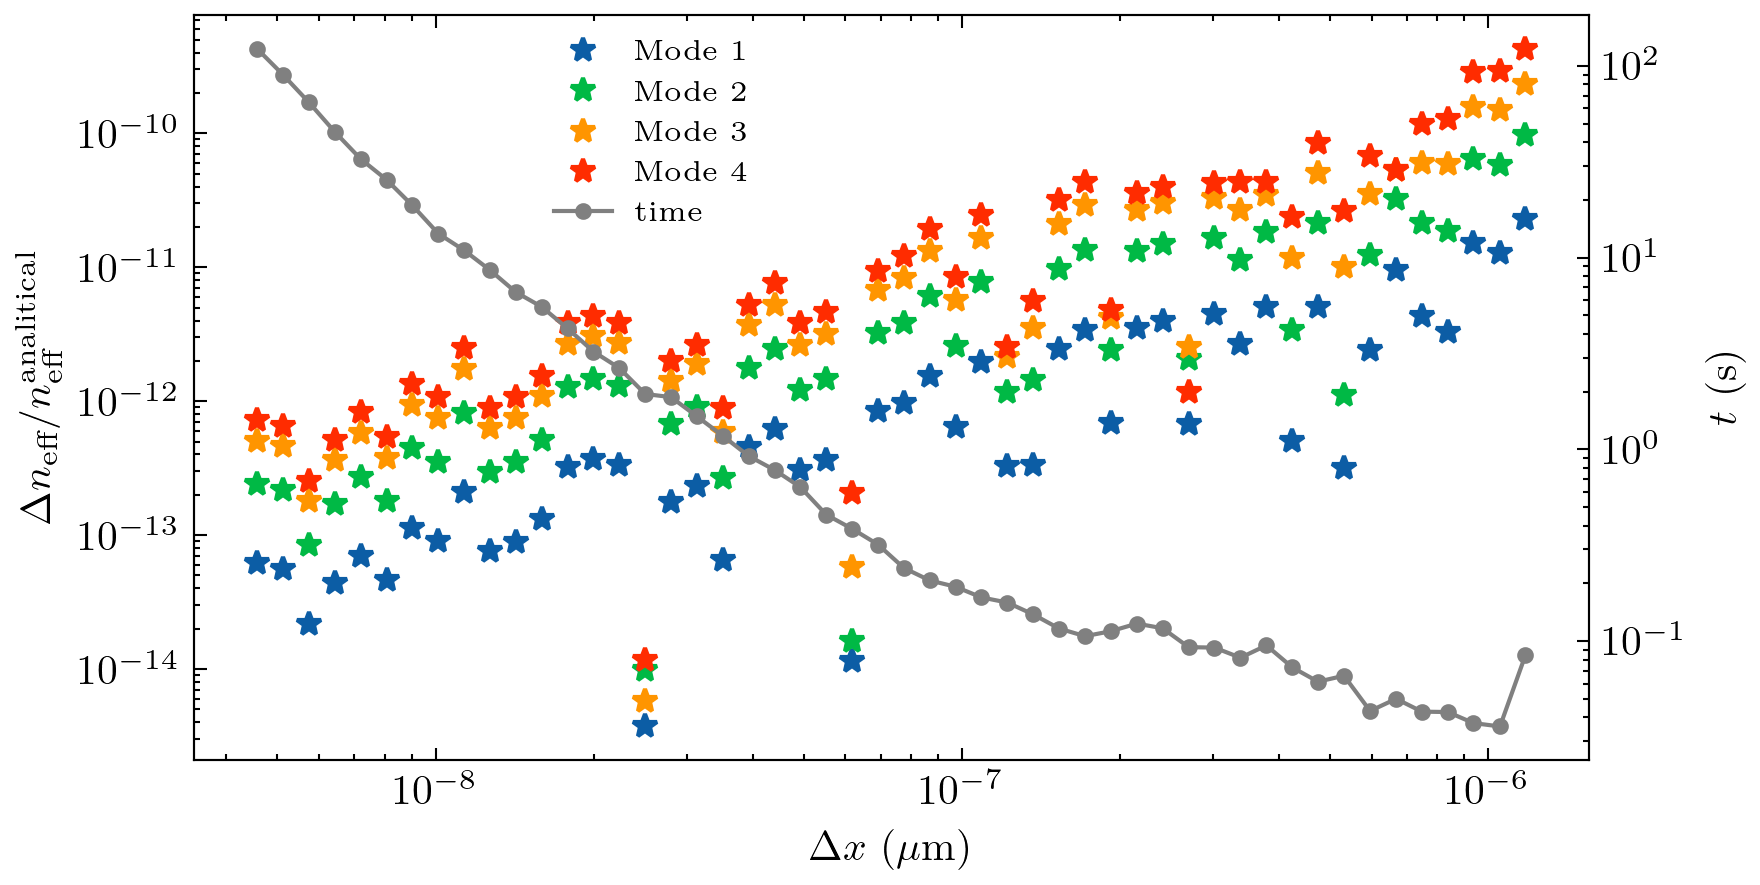
\includegraphics[width=\linewidth]{media/numerical_slab}
	\caption[Error relativo y tiempo de ejecución.]{Error relativo y tiempo de ejecución de las soluciones numéricas a la ecuación (\ref{eqn:eme}) con respecto a las soluciones analíticas, en función del paso $\Delta x$. \label{fig:emenumerror}}
\end{figure}
\section{Beam Propagation Method} 

Otra forma de abordar la integración numérica de la ecuación (\ref{eqn:helmholtznum}) consiste en separar el campo en su envolvente lenta y una fase rápidamente oscilante, considerando que en el rango visible el orden de magnitud es, $k_0 \sim 10 ^{5} \text{ cm}^{-1}$: $\Psi(\textbf{r}) = \phi(x,y,z)\exp(ik_0 n_0 z)$. Luego de reemplazar en la ecuación (\ref{eqn:helmholtznum}) se obtiene la ecuación óptica de Schrödinger \citep{paraxialschrodinger}:

\begin{equation}
	-2ik_0 n_0\frac{\partial }{\partial z}\phi(x,y, z) =  \left[\nabla_\perp^2 + k_0^2 (n^2(\textbf{r})-n_0^2)\right]\phi(x,y, z), \label{eqn:bpmescalar}
\end{equation} 
donde se ha utilizado la aproximación paraxial $\left| \frac{\partial^2 \phi}{\partial z^2} \right| \ll 2 k_0 n_0\left| \frac{\partial \phi}{\partial z} \right|$. Los algoritmos que resuelven la ecuación (\ref{eqn:bpmescalar}) son conocidos como \textit{Beam Propagation Methods} escalares, utilizados ampliamente en esta área de investigación \cite{bics, interorbital, OAMCaging, vortex, bpm}. Fuera de la aproximación de guiaje débil, los efectos de polarización cruzada son más relevantes y se hace necesaria una descripción vectorial del problema.
\subsection{Implementación mediante transformada de Fourier (FFTBPM)}
La ecuación (\ref{eqn:bpmescalar}) se puede escribir en términos de operadores lineales como \citep{bpm}: 
\begin{equation}
	\frac{\partial \phi}{\partial z}  = \left(\hat{A} + \hat{B}\right)\phi, \text{ con } \hat{A} \equiv i\frac{\nabla^2_\perp}{2k_0n_0}\text{ y } \hat{B} \equiv i\frac{k_0}{2n_0}\left[n^2(\textbf{r})-n_0^2\right]. \label{eqn:bpmop}
\end{equation}

La solución formal a la ecuación (\ref{eqn:bpmop}) es $\phi(\textbf{r}) = \exp\left[\left(\hat{A} + \hat{B}\right)(z-z_0)\right]\phi(x, y, z_0)$. Es conveniente trabajar con el operador $\hat{A}$ en el espacio de Fourier y con el operador $\hat{B}$ en el espacio directo. Dado que $\hat{A}$ y $\hat{B}$ no conmutan en general, se puede expandir el operador exponencial a orden $O(\Delta z ^3)$ como $\exp\left[\left(\hat{A} + \hat{B}\right)\Delta z \right] \approx \exp\left(\frac{\hat{A}\Delta z}{2} \right)\exp\left(\hat{B}\Delta z \right)\exp\left(\frac{\hat{A}\Delta z}{2} \right) + O(\Delta z ^3)$.

El algoritmo a implementar es el siguiente:
\begin{enumerate}
	\item   Se comienza con un perfil $\phi(x, y, z_0)$
\item   Se actúa en el espacio de Fourier transformando el perfil y multiplicado por la fase asociada a $\hat{A}$: $\exp\left(\frac{ik^2\Delta z}{4k_0 n_0}\right)\mathcal{F}(\phi(z_0))$, donde $k=\sqrt{k_x^2 + k_y^2}$ son las frecuencias de Fourier.
\item   Se aplica transformada de Fourier inversa y se multiplica por la fase asociada a $\hat{B}$: 

$\exp\left[\frac{i\Delta z k_0^2(n^2-n_0^2)}{2 k_0n_0}\right]\mathcal{F}^{-1}\left(\exp\left(\frac{ik^2 \Delta z}{4k_0 n_0}\right)\mathcal{F}(\phi(z_0))\right)$
\item  Se regresa al espacio de Fourier y se multiplica por la fase asociada a $\hat{A}$:
 
$\exp\left(\frac{ik^2\Delta z}{4k_0 n_0}\right)\mathcal{F}\left\{\exp\left[\frac{ik_0^2(n^2-n_0^2)}{2 k_0n_0}\Delta z \right]\mathcal{F}^{-1}\left[\exp\left(\frac{ik^2\Delta z}{4k_0 n_0}\right)\mathcal{F}(\phi(z_0))\right]\right\}$
\item Se vuelve al espacio real, habiendo avanzado un paso $\Delta z$:

$\phi(z_0+\Delta z)=\mathcal{F}^{-1}\left\{\exp\left(\frac{ik^2\Delta z}{4k_0 n_0}\right)\mathcal{F}\left\{\exp\left[\frac{i k_0^2(n^2-n_0^2)}{2 k_0n_0}\Delta z\right]\mathcal{F}^{-1}\left[\exp\left(\frac{ik^2\Delta z}{4k_0 n_0}\right)\mathcal{F}(\phi(z_0))\right]\right\} \right\}$

\item Se itera hasta llegar a la distancia de propagación $z$ deseada.
\end{enumerate}
En la Figura \ref{fig:num-exp-comp} se comparan los perfiles de salida experimental y numérico, alcanzando una similtud razonable. 
\begin{figure}[H]
	\centering
	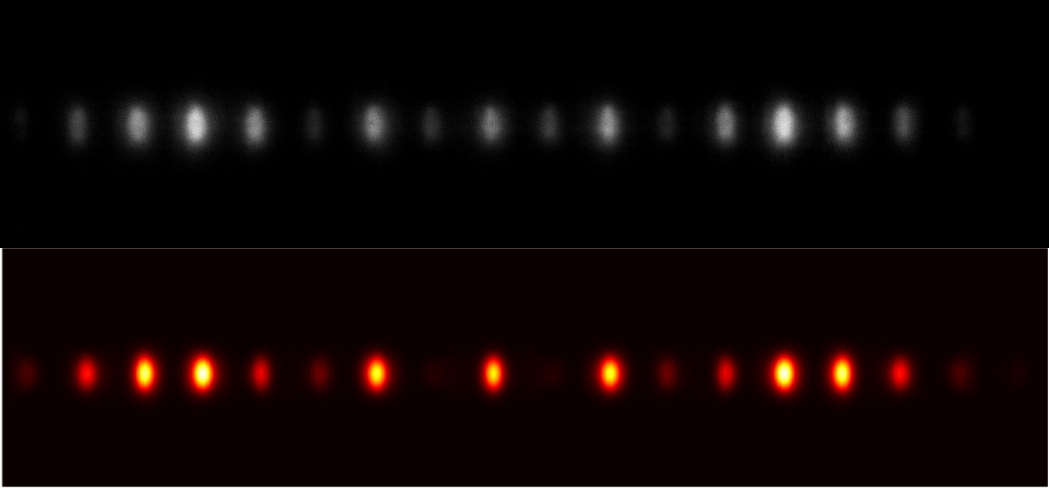
\includegraphics[width=0.7\linewidth]{media/num_exp_comparison.png}
	\caption{Comparación entre simulación y experimento. Arriba: Experimento. Abajo: Propagación numérica. \label{fig:num-exp-comp}}
\end{figure}



\section{Desde teoría de modos acoplados}
Se puede decir que la simulación numérica de las ecuaciones (\ref{eqn:non-ortho-CMT-eqs}) es lo más compacta posible en tanto la matriz de acoplamientos $\hat{C}$ codifica todas las propiedades de la red que se deseen estudiar de manera semiempírica. En este sentido, la diagonalización de la matriz $\hat{C}$ es una herramienta numérica útil en el estudio del comportamiento de redes fotónicas ante variaciones de parámetros tales como la dimerización (razón entre dos constantes de acoplamiento) o el desintonizado (diferencia entre constantes de propagación de dos modos distintos). Incluso, es posible explorar sistemas ``no físicos'' debido a los grados de libertad en las entradas de la matriz $\hat{C}$.